\begin{figure}[h]
  \centering
%segundo bloco de figuras
  \begin{tabular}{p{10cm} p{2cm} p{10cm}}
   \centering 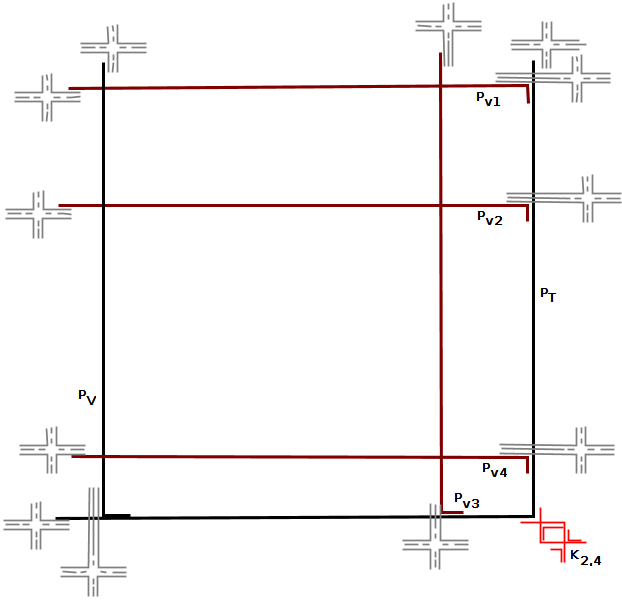
\includegraphics[width=10cm, left]{./img/gf3.png} & & 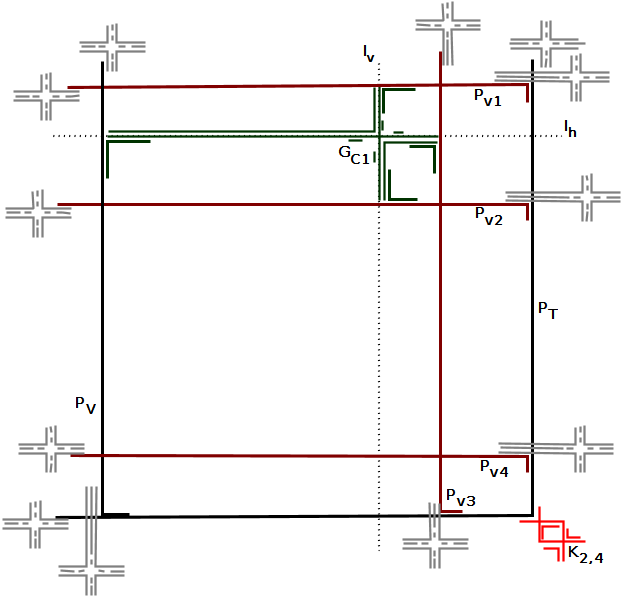
\includegraphics[width=10cm, left]{./img/formulaCompletaGFonePiePlusLines.png} \\  
  [\abovecaptionskip]
    \footnotesize \centering (a) Representação com dispositivos cláusula omitidos & & \footnotesize(b) Representação  com  $G_{C_1}$  associado com a cláusula $(x_1+x_2+x_3)$ em destaque \\
  \end{tabular}

 \caption{Representação de dobra simples dos dispositivos base e variáveis associados com as atribuições $x_1=False, x_2=False, x_3=True, x_4=False$} \label{fig:gadgetOnePie} \label{fig:gadgetBasePlusVariables}
\end{figure}